\documentclass{beamer}\usepackage[]{graphicx}\usepackage[]{color}
%% maxwidth is the original width if it is less than linewidth
%% otherwise use linewidth (to make sure the graphics do not exceed the margin)
\makeatletter
\def\maxwidth{ %
  \ifdim\Gin@nat@width>\linewidth
    \linewidth
  \else
    \Gin@nat@width
  \fi
}
\makeatother

\definecolor{fgcolor}{rgb}{0.345, 0.345, 0.345}
\newcommand{\hlnum}[1]{\textcolor[rgb]{0.686,0.059,0.569}{#1}}%
\newcommand{\hlstr}[1]{\textcolor[rgb]{0.192,0.494,0.8}{#1}}%
\newcommand{\hlcom}[1]{\textcolor[rgb]{0.678,0.584,0.686}{\textit{#1}}}%
\newcommand{\hlopt}[1]{\textcolor[rgb]{0,0,0}{#1}}%
\newcommand{\hlstd}[1]{\textcolor[rgb]{0.345,0.345,0.345}{#1}}%
\newcommand{\hlkwa}[1]{\textcolor[rgb]{0.161,0.373,0.58}{\textbf{#1}}}%
\newcommand{\hlkwb}[1]{\textcolor[rgb]{0.69,0.353,0.396}{#1}}%
\newcommand{\hlkwc}[1]{\textcolor[rgb]{0.333,0.667,0.333}{#1}}%
\newcommand{\hlkwd}[1]{\textcolor[rgb]{0.737,0.353,0.396}{\textbf{#1}}}%

\usepackage{framed}
\makeatletter
\newenvironment{kframe}{%
 \def\at@end@of@kframe{}%
 \ifinner\ifhmode%
  \def\at@end@of@kframe{\end{minipage}}%
  \begin{minipage}{\columnwidth}%
 \fi\fi%
 \def\FrameCommand##1{\hskip\@totalleftmargin \hskip-\fboxsep
 \colorbox{shadecolor}{##1}\hskip-\fboxsep
     % There is no \\@totalrightmargin, so:
     \hskip-\linewidth \hskip-\@totalleftmargin \hskip\columnwidth}%
 \MakeFramed {\advance\hsize-\width
   \@totalleftmargin\z@ \linewidth\hsize
   \@setminipage}}%
 {\par\unskip\endMakeFramed%
 \at@end@of@kframe}
\makeatother

\definecolor{shadecolor}{rgb}{.97, .97, .97}
\definecolor{messagecolor}{rgb}{0, 0, 0}
\definecolor{warningcolor}{rgb}{1, 0, 1}
\definecolor{errorcolor}{rgb}{1, 0, 0}
\newenvironment{knitrout}{}{} % an empty environment to be redefined in TeX

\usepackage{alltt}
\usepackage{xcolor}
\usepackage{graphicx}
\usepackage{tikz}
\usetikzlibrary{shapes.geometric, arrows}
\usepackage{verbatim}
\definecolor{HTGorange}{RGB}{235,114,28}
\definecolor{HTGblue}{RGB}{50,155,219}

\useoutertheme{infolines}%makes informative footer
\usetheme{Pittsburgh}
\setbeamercolor{structure}{fg=HTGblue}
\setbeamercolor{normal text}{fg=black}
\setbeamercolor{upper separation line head}{bg=HTGorange}
\AtBeginSection{\frame{\sectionpage}}%make section title pages
\AtBeginSubsection{\frame{\subsectionpage}}

\setbeamertemplate{headline}
{
  \leavevmode
  \hbox{
  \begin{beamercolorbox}[wd=.5\paperwidth,ht=6ex,dp=2ex,left,rightskip=1em]{section in head/foot}%
    \usebeamerfont{subsection in head/foot}\hspace*{2ex}\insertshorttitle
  \end{beamercolorbox}
  \begin{beamercolorbox}[wd=.25\paperwidth,ht=6ex,dp=1ex,left,leftskip=1em]{subsection in head/foot}%
    \usebeamerfont{section in head/foot}\insertsectionhead\hspace*{2ex}
  \end{beamercolorbox}
  \begin{beamercolorbox}[wd=.25\paperwidth,ht=6ex,dp=1ex,right,leftskip=1em]{subsection in head/foot}%
    
\includegraphics[scale=.15]{./Figures/HTGLogo.jpg}
  \end{beamercolorbox}}
  \begin{beamercolorbox}[colsep=1.5pt,ht=.75ex]{upper separation line head}
  \end{beamercolorbox}
  \vskip0pt%
}

\setbeamertemplate{footline}
{
  \leavevmode
  \hbox{%

\begin{beamercolorbox}[wd=.70\paperwidth,ht=4.25ex,dp=4ex,left,leftskip=2ex]{title in head/foot}%
    \usebeamerfont{title in head/foot}\insertshorttitle{} - \insertshortauthor
\end{beamercolorbox}%
\begin{beamercolorbox}[wd=.20\paperwidth,ht=4.25ex,dp=4ex,center]{date in head/foot}%
    \usebeamerfont{date in head/foot}\insertshortdate{}
\end{beamercolorbox}%
\begin{beamercolorbox}[wd=.10\paperwidth,ht=4.25ex,dp=4ex,right,rightskip=2ex]{date in head/foot}%
    \insertframenumber{} / \inserttotalframenumber
  \end{beamercolorbox}}%
\vskip0pt%
}



\setbeamertemplate{frametitle}{%place the title in the center

\vspace*{4mm}\hspace*{-2mm}\insertframetitle

}


\setbeamertemplate{navigation symbols}{}%remove Navigation Symbols
%start entering presentation specific stuff below here...
%start entering presentation specific stuff below here...%%%%%%%%%%%%%%%%%%%%%%%%%%%%%%%%%%%%%%%%%%%%%%%
\tikzstyle{startstop} = [rectangle, rounded corners, minimum width=3cm, minimum height=1cm,text centered, draw=black, fill=blue!30]
\tikzstyle{io} = [trapezium, trapezium left angle=70, trapezium right angle=110, minimum width=3cm, minimum height=1cm, text centered, draw=black, fill=blue!20]
\tikzstyle{process} = [rectangle, minimum width=3cm, minimum height=1cm, text centered, draw=black, fill=orange!30]
\tikzstyle{decision} = [diamond, minimum width=3cm, minimum height=1cm, text centered, draw=black, fill=green!30]
\tikzstyle{arrow} = [thick,->,>=stealth]
\tikzstyle{doublearrow} = [thick,<->,>=stealth]

\title[Reproducible Research Tools]{Reproducible research tools to increase efficiency and reduce errors}
\author[Dominic LaRoche]{Dominic LaRoche}
\IfFileExists{upquote.sty}{\usepackage{upquote}}{}
\begin{document}

\maketitle
\begin{frame}{Outline}
\begin{itemize}
\item Introduction and Motivation
\item The Tools of the Trade
\item Examples
\item Benefits to You and HTG
\end{itemize}
\end{frame}

\section{Introduction}

\begin{frame}{What is Reproducible Research?}
What does it mean to have ``reproducible" research?\\
\pause
\vspace{.5cm}
We break research down into 2 phases:\\
\pause
\begin{itemize}
\item[1.)] Data generating experiment
  \begin{itemize}
  \item Can the same data be generated again?
  \item This is an ongoing topic in the annals of \emph{Nature} and \emph{Science}
  \end{itemize}
\pause
\bigskip
\item[2.)] Can the analysis and results be reproduced given the same data?
  \begin{itemize}
  \item The focus of my talk today
  \pause
  \item Three questions:
    \begin{itemize}
    \item[1.)] Can you reproduce the results right now?
    \item[2.)] Can you reproduce the results a year from now?
    \item[3.)] Can someone else reproduce the results in 5 years?
    \end{itemize}
  \end{itemize}
\end{itemize}
\end{frame}

\begin{frame}{Why Reproducible Research?}
This is the alternative!

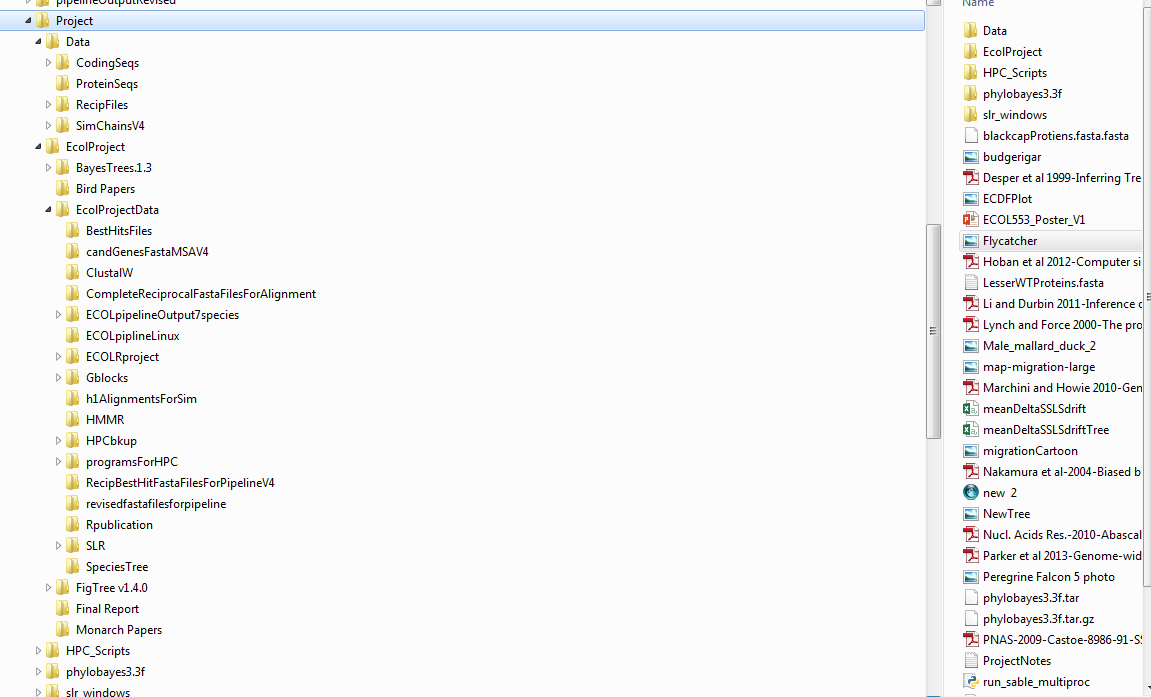
\includegraphics[scale=.25]{./Figures/FolderMess.png}\\
\pause
I dare you to try and reproduce my results!\\
(or check them for accuracy)\\
\end{frame}

\begin{frame}{The Change Cascade}
What if I need to make a change?\\
\pause

\begin{itemize}
\item Noticed an error\\
\item Received new or additional data\\
\end{itemize}

\pause
\vspace{.5cm}
How many different places do I need to update?\pause $\rightarrow$ \textcolor{red}{\emph{Wasted Time}\\}

\pause
\begin{center}
\rule{8cm}{.5pt}\\
\end{center}
\vspace{.2cm}
What if we need to make a change in a year (or two)?\\

\pause
\vspace{0.5cm}
\textcolor{red}{What did I do again???}
\end{frame}



\begin{frame}{Elements of Reproducibility}
What do we need to do to make analyses reproducible?
\bigskip
\pause
\begin{itemize}
\item Organization (where are my car keys?)
\pause
  \begin{itemize}
  \item Standard folder structure and naming conventions
  \item Code--Report pairing
  \end{itemize}
\pause  
\bigskip
\item Literate Programming
  \begin{itemize}
  \item Well documented code
  \item ``Human readable"
  \end{itemize}
\pause
\bigskip
\item Version control
  \begin{itemize}
  \item Tracked changes from project inception
  \item software and package versions controlled
  \end{itemize}
\end{itemize}

\end{frame}

\section{The Vision}

\begin{frame}{The Tools}
We can use tools to help with organization and version control
\pause
\bigskip
\begin{itemize}
\item Organization 
  \begin{itemize}
  \item \LaTeX\ or Rmarkdown typesetting language + knitr (with R studio)
  \item HTG R Package
  \end{itemize}
\pause  

\bigskip
\item Version control
  \begin{itemize}
  \item Git
  \item Checkpoint
  \end{itemize}
\end{itemize}
\bigskip
\pause
Use these tools together to create a seamless analysis $\rightarrow$ report pipeline.\\

\end{frame}

\begin{frame}{System Overview}

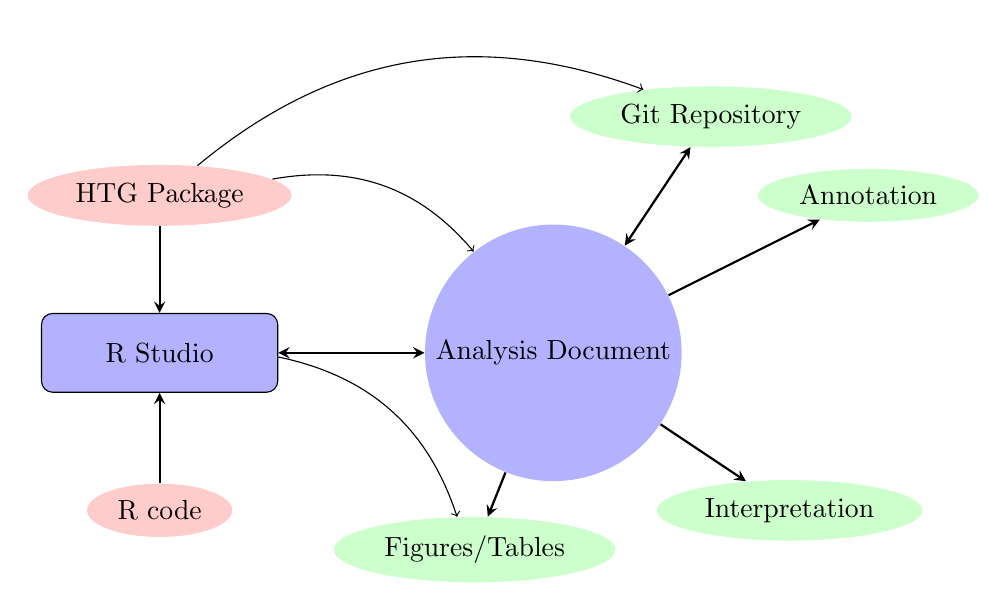
\begin{tikzpicture}[node distance=2cm]
\node (start) [startstop] {R Studio};
\node[fill=red!20, ellipse, below of=start](codein){R code};
\node[fill=red!20, ellipse, above of=start](pack){HTG Package};
\draw [arrow] (codein)--(start);
\draw [arrow] (pack)--(start);
\pause
\node [fill=green!20, ellipse, right of=pack,xshift=5cm,yshift=1cm](repo){Git Repository};
\path[->] (pack) edge [bend left] (repo);
\pause

\node[fill=blue!30,circle,right of=start,xshift=3cm] (mainout) {Analysis Document};
\path[->] (pack) edge [bend left] (mainout);
\pause

\draw [doublearrow] (start)--(mainout);
\pause
\draw [doublearrow] (repo)--(mainout);
\pause
\node [fill=green!20, ellipse, right of=codein,xshift=2cm,yshift=-.5cm](figtab){Figures/Tables};
\draw [arrow] (mainout)--(figtab);
\pause

\node [fill=green!20, ellipse, right of=repo,yshift=-1cm](anoteout){Annotation};
\draw [arrow] (mainout)--(anoteout);
\pause
\node [fill=green!20, ellipse, right of=figtab,xshift=2cm,yshift=.5cm](interp){Interpretation};
\draw [arrow] (mainout)--(interp);
\pause
\path[->] (start) edge [bend left](figtab);

\end{tikzpicture}
\end{frame}


\subsection{The Tools}
\begin{frame}{R-Studio}
R-Studio is a friendly code editor :\\
\begin{itemize}
\item Built in  editor support for:
  \begin{itemize}
  \item R code
  \item C++
  \item JavaScript
  \item CSS
  \item DCF
  \item Markdown
  \item HTML
  \item Tex
  \item Python
  \end{itemize}
\item It can also handle:
  \begin{itemize}
  \item PERL
  \item SAS ...etc
  \end{itemize}
\item Can enable emacs key-bindings
\end{itemize}
\end{frame}

\begin{frame}{R-Studio}
R-Studio combined with \LaTeX or Rmarkdown can make:\\
\begin{itemize}
\item Reports
\item Articles (formatted to most journals)
\item Presentations
\item Web pages and more...
\end{itemize}
\pause
\bigskip
(This presentation was made with R-studio)
\end{frame}

\begin{frame}{Git}
Git is a version control system that also works with Rstudio
\bigskip
\begin{itemize}
\item Tracks changes to all documents in the folder or subfolders
  \begin{itemize}
  \item This includes figures, pictures, emails, etc.
  \end{itemize}
\pause
\item Can retrieve any previous version of a file
\pause 
\item No need to create multiple copies of a document
\pause
  \begin{itemize}
  \item Changes are tracked through commits
  \pause
  \item Each commit is attached to a (detailed) message about the changes/ status of the document
  \end{itemize}
  \pause
\item Can make ``clones" so that anyone can get the most current version of everything with a single command
\pause
\item Can specify items you don't want tracked
\pause
\item Can ``Fork" a project into a new project
\end{itemize}
\end{frame}

\begin{frame}{Checkpoint}
Checkpoint is an R package to keep track of package versions
\bigskip
\begin{itemize}
\item Git doesn't track changes to the computing environment
\pause
\item Checkpoint creates a snapshot of all R packages used in the analysis
\pause
\item Package versions are maintained on a separate server (using a git style change tracker).
\pause
\item Can access the working version of any CRAN package at any time
  \begin{itemize}
  \item No need to worry that, \emph{ahem}, someone is using a really old version of the package
  \item Can keep your system up-to-date without worrying about breaking an analysis
  \end{itemize}

\end{itemize}
\end{frame}

\begin{frame}{HTG Private Package}
The HTG package eases implementation of reproducible research
\bigskip
\begin{itemize}
\item MakeProject()
  \begin{itemize}
  \item Single command creates version controlled project folder
  \item Creates analysis/report templates with either Rmarkdown or \LaTeX
  \item Creates README file for the project to facilitate communication and collaboration
  \item Creates Rproject file
  \end{itemize}
  \pause
\item CloneProject()
  \begin{itemize}
  \item Clones existing version controlled project to your computer
  \end{itemize}
  \pause
\item Can be a place to keep other standard functions 
\end{itemize}
\end{frame}


\begin{frame}{The Glue}
R-studio makes it easy to implement these tools
\bigskip
\begin{itemize}
\item Weaves code and text together to make reports 
\bigskip
  \begin{itemize}
  \item Works with Rmarkdown or \LaTeX
  \smallskip
  \item Rmarkdown lowers the bar for making reports
  \end{itemize}
\bigskip
\pause
\item Has easy interface with Git
  \begin{itemize}
  \item Can see change history and associated hashes
  \item has simple pull, commit and push cammands etc.
  \end{itemize}
\end{itemize}
\end{frame}

\begin{frame}{Outside Groups}
How do we maintain reproducibility outside our group?
\pause
Shiny applications
\begin{itemize}
\item Provide easy-to-use program to perform a specific task
\item Eliminates use of other programs and click-through analyses
\item Can incorporate documentation (exported code and report)
\item Demo...
\end{itemize}
\end{frame}




\section{Conclusions}



\begin{frame}{Benefits}
\begin{itemize}
\item Standardized file structure
\bigskip
\item Access to all previous versions of everything
\bigskip
\item HTG package eases set-up and saves time
\bigskip
\item Anyone can pick up where you left off or find important figures and documents
\end{itemize}
\end{frame}

\begin{frame}
\begin{columns}
\begin{column}{.6\textwidth}
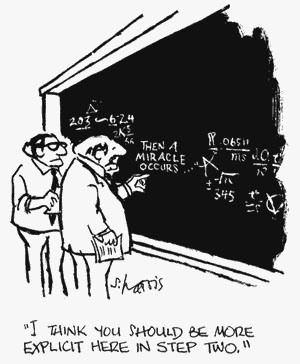
\includegraphics[scale=.5]{./Figures/Cartoon}
\end{column}

\begin{column}{.4\textwidth}
\huge{Questions?}
\end{column}
\end{columns}

\end{frame}


\end{document}
